\chapter{The Standard Model of Particle Physics}\label{ch:sm}

The Standard Model is a set of theories describing the interactions between elementary particles.
It explains three of the four known fundamental forces, namely the electromagnetic force,
the weak nuclear force, and the strong force.
It does not include  or account for gravitational interactions.

The Standard Model can be fairly characterized as one of the most successful theories in science.
A huge number of predictions made by the theory have been confirmed experimentally,
some to an astounding degree of accuracy.
Precision measurements of the magnetic moment of the electron have shown the experimental and theoretical values of the
fine structure constant to agree better than one part in one billion.\cite{sm-fine-structure-2008}
The ATLAS detector at the LHC has confirmed the predicted rate of particle production for a very wide range of
production processes and final states.
A summary of Standard Model measurements made by ATLAS, and their comparisons to theoretical predictions can be seen in figure~\ref{fig:sm_xsec_summary}.
The Standard Model predicted the existence of the W boson, the top quark, and the Higgs boson,
which were all later confirmed by experiment.

\begin{figure}[h!]
    \centering
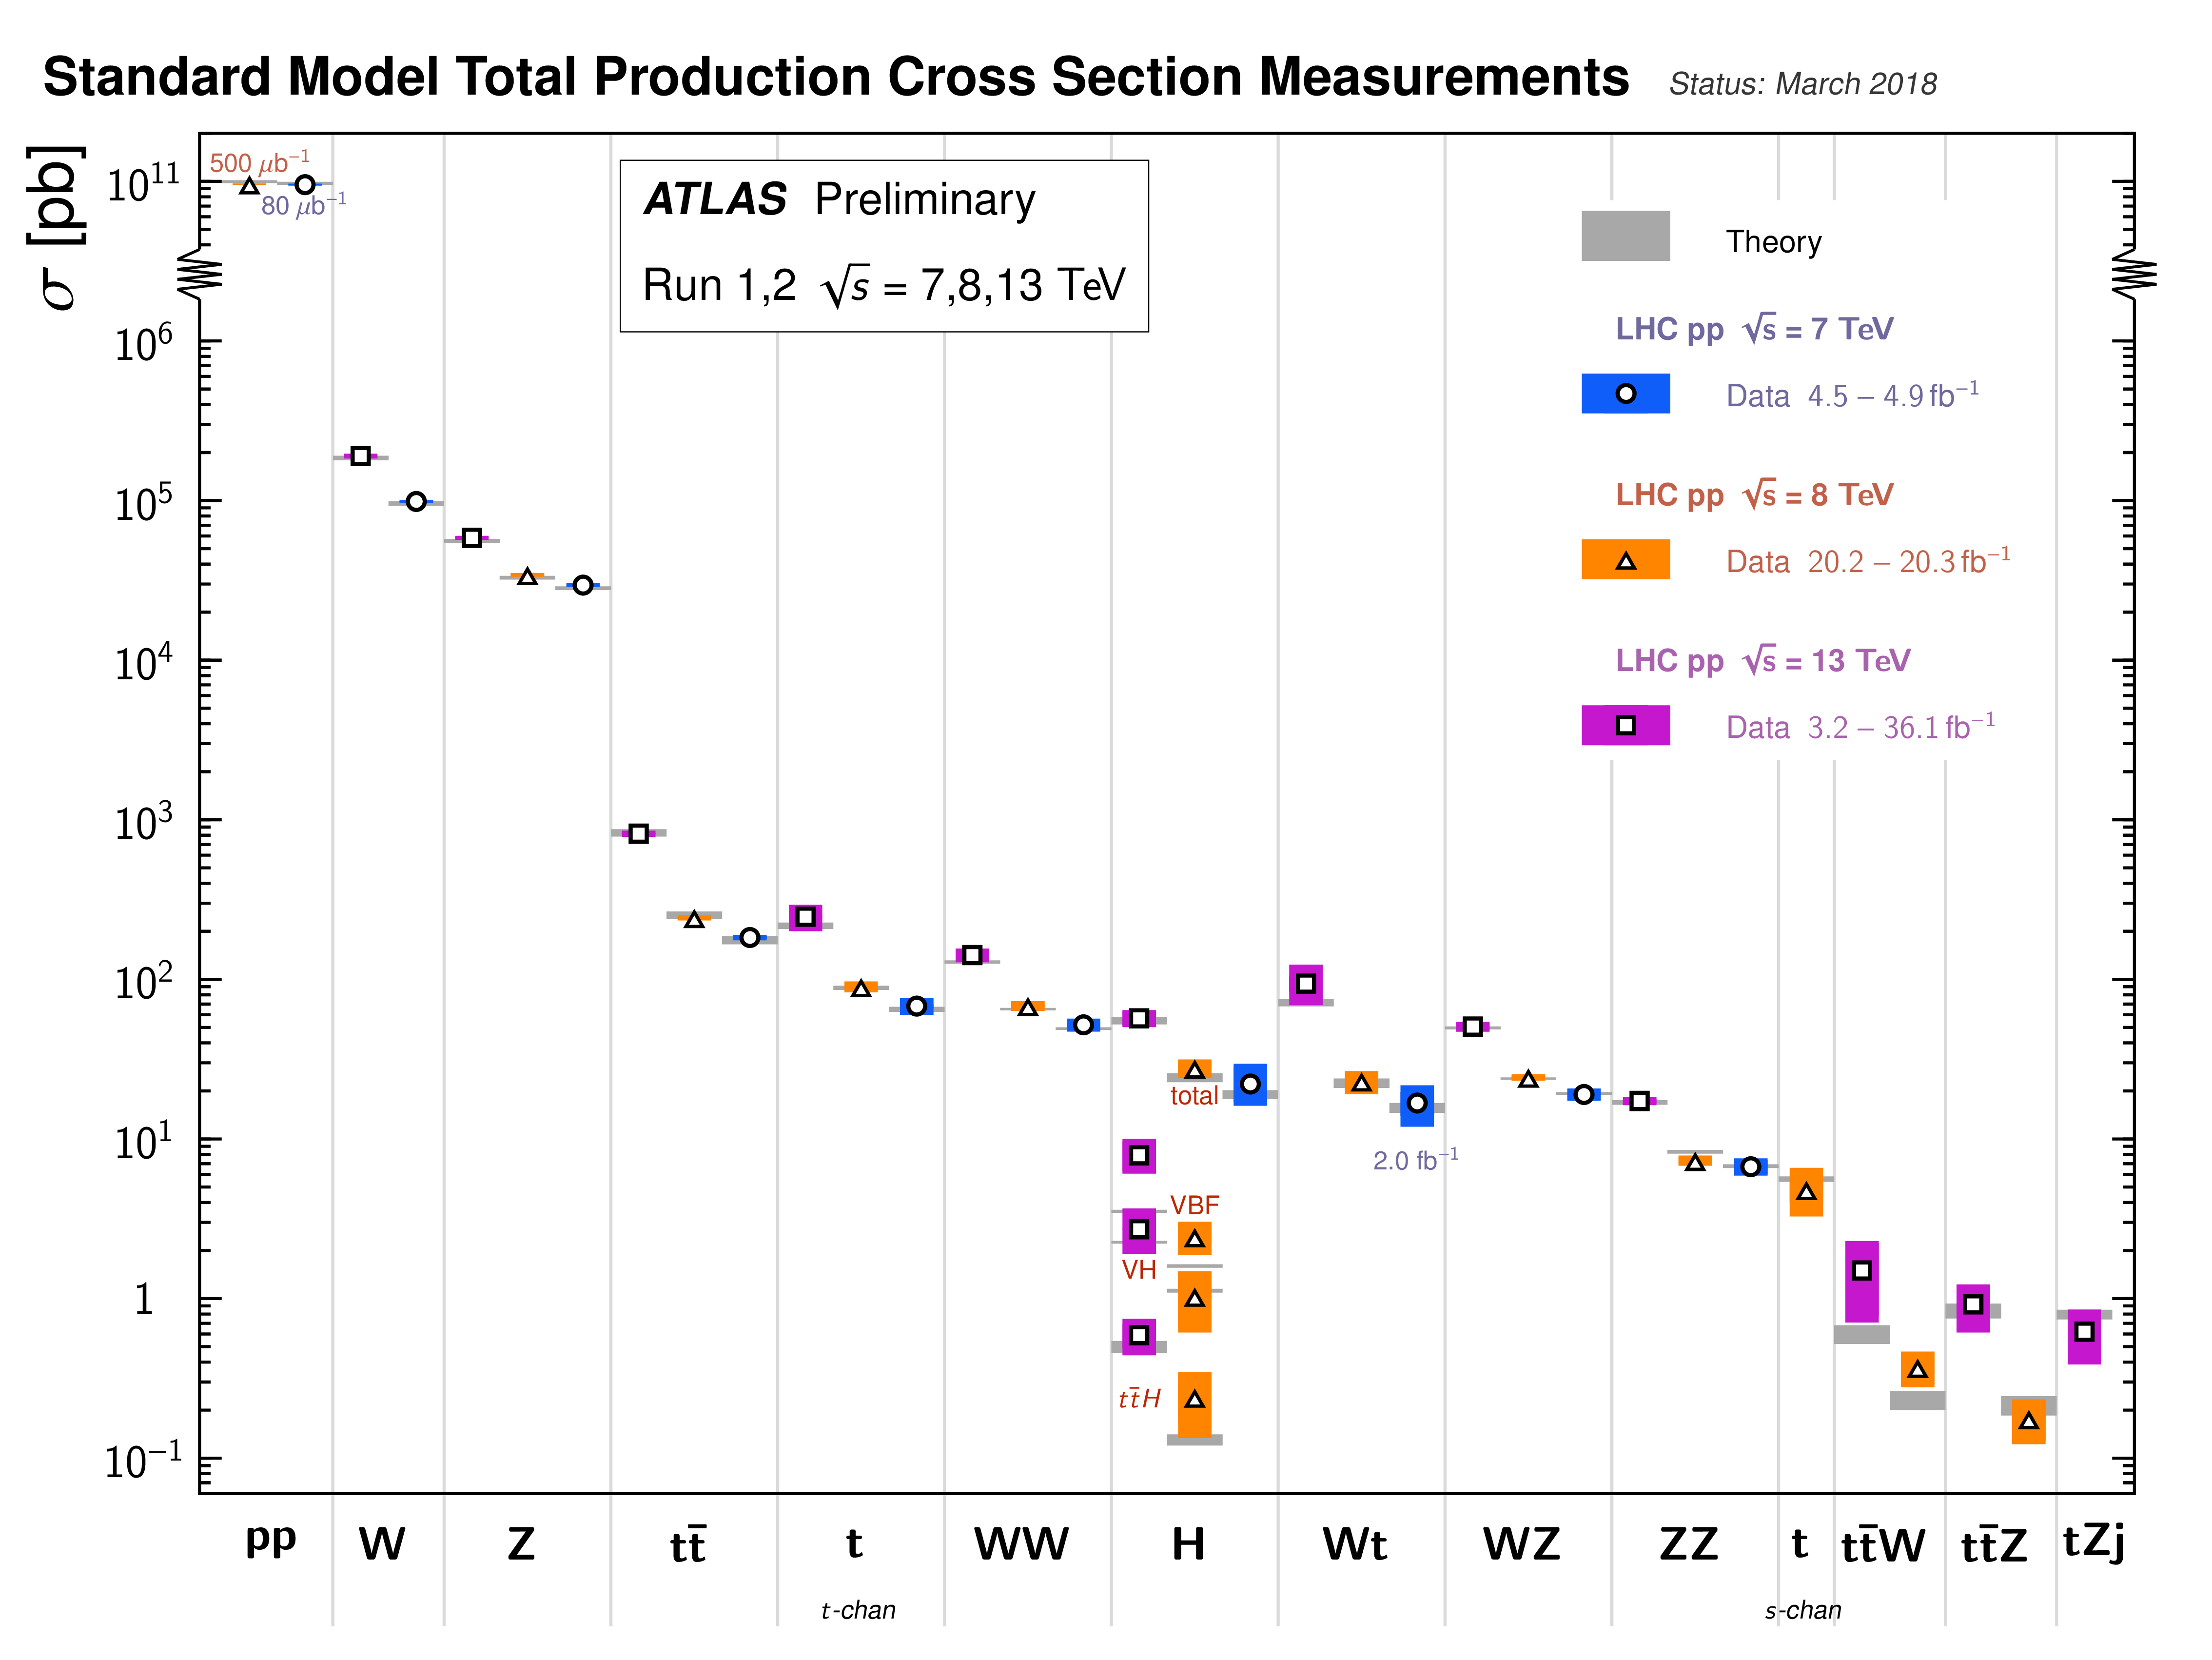
\includegraphics[width=0.6\linewidth]{sm_xsec_summary}
\caption{Summary of Standard Model production cross sections measured by ATLAS, compared to theoretical predictions.}
\label{fig:sm_xsec_summary}
\end{figure}

The Standard Model is expressed in the language of Quantum Field Theory.
The theory consists of three generations of matter fields,
specified by their representation under the gauge group $SU(3)\times SU(2)\times U(1)$ and the Poincar\'e group,
as well as a complex scalar field.
Poincar\'e symmetry consists of the Lorentz symmetry of special relativity, plus global translational symmetry.

The Standard Model is a complete theory in the sense that it is internally self-consistent,
and all particles predicted by the theory have been discovered experimentally.
However, the Standard Model does not account for all known physical phenomena,
and so cannot be considered a complete theory of nature.

\section{Electroweak Sector and the Higgs Mechanism}\label{sec:sm_ew}

\subsection{Matter fields}\label{subsec:ew_fields}

All left-handed matter fields are $SU(2)$ doublets, while their corresponding right-handed fields are $SU(2)$ singlets.
There are three generations of left-handed lepton fields:

\begin{equation}\label{eq:left_handed_leptons}
    \psi_L =
    \begin{pmatrix}
        \nu_e \\ l_e
    \end{pmatrix}_L,\;
    %
    \begin{pmatrix}
        \nu_{\mu} \\ l_{\mu}
    \end{pmatrix}_L,\;
    %
     \begin{pmatrix}
        \nu_{\tau} \\ l_{\tau}
    \end{pmatrix}_L
\end{equation}

And three generations of right-handed lepton fields:
\begin{equation}\label{eq:right_handed_leptons}
\psi_R = e_R,\; \mu_R,\; \tau_R
\end{equation}

Similarly, there are three generations each of the left-handed $SU(2)$-doublet quark fields,
each of which comes in three colors:

\begin{equation}\label{eq:left_handed_quarks}
   \psi_L =
    \begin{pmatrix}
        q_u \\ q_d
    \end{pmatrix}_L,\;
    %
    \begin{pmatrix}
        q_{c} \\ q_{s}
    \end{pmatrix}_L,\;
    %
     \begin{pmatrix}
        q_{t} \\ q_{b}
    \end{pmatrix}_L
\end{equation}

Quark color will play a role in QCD interactions, as discussed in the next session.
There are also the corresponding $SU(2)$-singlet right-handed fields:

\begin{equation}\label{eq:right_handed_quarks}
\psi_R = q_{uR},\; q_{dR},\; q_{cR},\; q_{sR},\; q_{tR},\; q_{bR}
\end{equation}

\subsection{Symmetries and Lagrangian}\label{subsec:ew_lagrangian}
The symmetry constraining the electroweak sector of the Standard Model Lagrangian is $SU(2)_L \times U(1)_Y$.
The subscript $L$ for the $SU(2)$ group indicates that it only acts on the left-handed fields in the theory.
As we've seen, right-handed fields appear as $SU(2)$ singlets.
The Lagrangian density satisfying the required symmetries, including all renormalizable terms, is:

\begin{equation}\label{eq:ew_lagrangian}
    \mathcal{L}_{EW} = \mathcal{L}_{kin} + \mathcal{L}_{\text{interactions}}
\end{equation}

The kinetic part of the electroweak Lagrangian is:

\begin{equation}\label{eq:ew_kin}
    \mathcal{L}_{kin} = -\frac{1}{4}W^{\mu \nu}_{a}W_{\mu \nu}^{a}-\frac{1}{4}B^{\mu \nu}B_{\mu \nu}
\end{equation}

Where $W_\mu^a$ are the three $SU(2)_L$ gauge bosons, $B_\mu$ is the $U(1)_Y$ (hypercharge) gauge boson,
and $W_\mu\nu = \partial_{\mu} W_{\nu} - \partial_{\nu} W_{\mu}$.

The part of the electroweak Lagrangian describing electroweak interactions is:

\begin{equation}\label{eq:ew_int}
    \mathcal{L}_{\text{interactions}} = \sum_{\text{generations}}\left[\frac{g}{2}\bar{\psi}_{L}\gamma^\mu\sigma^i W_\mu^i \psi_L+
    g'B_\mu\left(Y_{\psi_L}\bar{\psi}_L\gamma^\mu\psi_L + Y_{\psi_R}\bar{\psi}_R\gamma^\mu \psi_R\right)\right]
\end{equation}

Where $\gamma^\mu$ are the Dirac gamma matrices, Y is the hypercharge associated with the relevant field.
Left-handed leptons and quarks have weak hypercharge $Y = -1$ and $Y = 1/3$, respectively.
Right-handed leptons have weak hypercharge $Y = -2$, while right-handed up-type quarks have weak hypercharge $Y = 4/3$,
and right-handed down-type quarks have weak hypercharge $Y = -2/3$.

This Lagrangian describes the charged-current and neutral-current weak interactions, as well as weak gauge boson self-interactions.
However, it is insufficient to describe nature because the gauge bosons are massless in this theory.
It would be impossible to include gauge boson mass terms in the electroweak Lagrangian without explicitly breaking the symmetry.
Similarly, it's impossible to introduce Lorentz-invariant fermion mass terms that keep the Lagrangian invariant under $SU(2)_L \times U(1)_Y$.
In order to reconcile this theory with the experimentally observed fact of massive weak gauge bosons and massive fermions,
an entirely new field will have to be introduced.

\subsection{Spontaneous symmetry breaking}\label{subsec:ew_higgs}

The original $SU(2)_{L}\times U(1)_Y$ symmetry will be spontaneously broken, via the nonzero Higgs vacuum expectation value, to $U(1)_{QED}$.
This process of spontaneous symmetry breaking (SSB) generates fermion masses, electroweak gauge boson masses,
and the Yukawa coupling terms between fermions.
It also generates a new massive real scalar field, known as the Higgs field.

We introduce a new $SU(2)$-doublet complex scalar field, $\phi$, as well as a potential of the form:

\begin{equation}\label{eq:higgs_potential}
    V(\phi) = \mu^2 \phi^\dagger\phi + \lambda(\phi^\dagger\phi)^2
\end{equation}

With $\lambda > 0$ and $\mu^2 <0$.
The minimum energy state satisfies: $\phi^\dagger\phi = \frac{-\mu^2}{2\lambda}$.

We can then re-parameterize the scalar field as:

\begin{equation}\label{eq:higgs_param}
    \phi = \exp{\left(i\frac{\sigma_i}{2}\theta^i(x)\right)}\frac{1}{\sqrt{2}}\begin{pmatrix} 0 \\ v+H(x) \end{pmatrix}
\end{equation}

Where $H(x)$ and $\theta^i(x)$ are real-valued fields,
and $v = \sqrt{\frac{-\mu^2}{\lambda}}$ is the vacuum expectation value of the Higgs field.

Because of the $SU(2)_L$ symmetry of the theory, we are free to choose convenient values for $\theta_i(x)$,
without affecting the outcome of any observable predictions.
Selecting $\theta_i(x) = 0$, the additional kinetic term required in the Lagrangian is:

\begin{equation}\label{eq:higgs_kinetic}
    \Delta\mathcal{L}_{EW} = \left(D_{\mu}\phi\right)^{\dagger}\left(D_{\mu}\phi\right)
    =\frac{1}{2}\partial_{\mu}H \partial^{\mu}H + (v+H)^{2}\left(\frac{g^2}{4}W_\mu^\dagger W^\mu
    + \frac{g^2}{8\cos^2 {\theta_W}}Z_\mu Z^\mu\right)
\end{equation}

Where $W_\mu$ and $Z_\mu$ are mass eigenstates of the electroweak gauge fields,
linear combinations of the original $W_\mu^a$ and $B_\mu$.

This has added interaction terms between the Higgs field and the $W$ and $Z$ bosons,
as well as quadratic terms for these same bosons.
A quadratic term in the Lagrangian is physically the same as having a mass term in the Lagrangian.

So we find that the $W$ and $Z$ boson masses are:

\begin{equation}\label{eq:wz_masses}
    M_w = \frac{1}{2}vg,\; M_Z = \frac{M_W}{\cos{\theta_W}}
\end{equation}

Through SSB, electroweak gauge boson masses have been generated without requiring explicit mass terms in the Lagrangian.

The introduction of this scalar field and its associated potential will also generate fermionic mass terms,
couplings between the fermions and the scalar field, and a mass term for the scalar field itself.

Like with the gauge bosons, adding an explicit fermionic mass term would break the $SU(2)_L \times U(1)_Y$ symmetry of the theory.
However, the introduction of the new scalar field allows for additional terms in the Lagrangian,
which can be written, in unitary gauge, as:

\begin{equation}\label{ew:yukawa_lagrangian}
    L_Y = \frac{1}{\sqrt{2}}\left(v+H\right)\left(c_{1}\bar{d}d+c_2\bar{u}u+c_3\bar{e}e\right)
\end{equation}

Once again, after spontaneous symmetry breaking, there appear terms in the Lagrangian that are quadratic in the fields.
These are mass terms for the fermions, and like for the gauge bosons, the masses are proportional to the Higgs vacuum
expectation value.

\begin{equation}\label{ew:fermion_masses}
    m_d = -c_1\frac{v}{\sqrt{2}},\; m_u = -c_2\frac{v}{\sqrt{2}},\; m_e = -c_3\frac{v}{\sqrt{2}}
\end{equation}

Unlike for the gauge bosons, we find no testable relationship between the fermion masses,
since the coefficients are all free parameters of the theory.

The Higgs mechanism allows for the generation of masses for electroweak gauge bosons and for fermions without explicitly
breaking the original symmetry of the theory.
Additional consequences arising from the Higgs mechanism are the relationship between $Z$ and $W$ boson masses,
the existence of a new massive scalar field, and interactions between this field and the fermions and gauge bosons.
The massive particle associated with this field, the Higgs boson, was discovered in 2012 by the ATLAS and CMS collaborations.

\section{Quantum Chromodynamics}\label{sec:sm_qcd}

Quantum Chromodynamics (QCD) is the part of the Standard Model that concerned strong interactions.
The fields involved are the quark fields, which also participate in electroweak interactions.
In the case of QCD, the quarks are in the fundamental $\boldsymbol{3}$ representation of $SU(3)$.

\subsection{Symmetries and Lagrangian}\label{subsec:ew_lagrangian}

Like the electroweak theory, QCD is a non-Abelian gauge theory.
The Lagrangian is generated by positing the transformations under which the Lagrangian is invariant,
and including all terms that respect these symmetries.
For QCD, the symmetry group is $SU(3)$, yielding the following Lagrangian:

\begin{equation}\label{eq:qcd_lagrangian}
    \mathcal{L}_{QCD} = \sum_{generations}i\bar{\psi}D_\mu\gamma^\mu\psi-\frac{1}{4}G_{\mu\nu}^a G_a^{\mu\nu}
\end{equation}

Where

\begin{equation}\label{eq:qcd_deriv}
D_\mu = \partial_\mu - i g_s G_\mu^a T^a
\end{equation}

is the gauge-covariant derivative, $g_s$ is the strong coupling constant, $G_\mu^a$ are the eight gluon fields,
and $T^a$ are the infinitesimal generators of $SU(3)$.

The gluon field strength tensor, $G_{\mu\nu}^a$, is defined as:

\begin{equation}\label{eq:qcd_field_strength}
    G_{\mu\nu}^a = \partial_\mu G_\nu^a - g_s f^{abc} G_\mu^b G_\nu ^c
\end{equation}

Where $f^{abc}$ are the $SU(3)$ structure constants.

This Lagrangian describes the interactions between quarks and gluons, as well as the gluon self-interactions.

\subsection{QCD coupling constant}\label{subsec:qcd_coupling}

A consequence of the gluon self-interaction in the QCD Lagrangian is that the value of the strong coupling constant,
$g_s$, depends on the energy scale.
The rate of change of the coupling with increased energy is described by the $\beta$ function,

\begin{equation}\label{eq:sm_qcd_beta}
    \beta\left(\alpha_s\right) = \frac{\alpha_s}{2\pi}\left(\frac{11}{3}n_{\text{colors}}-\frac{4}{3}n_{\text{flavors}}\right)
\end{equation}

Where $\alpha_s = g_s^2 / 4\pi$.


\begin{figure}[h!]
    \centering
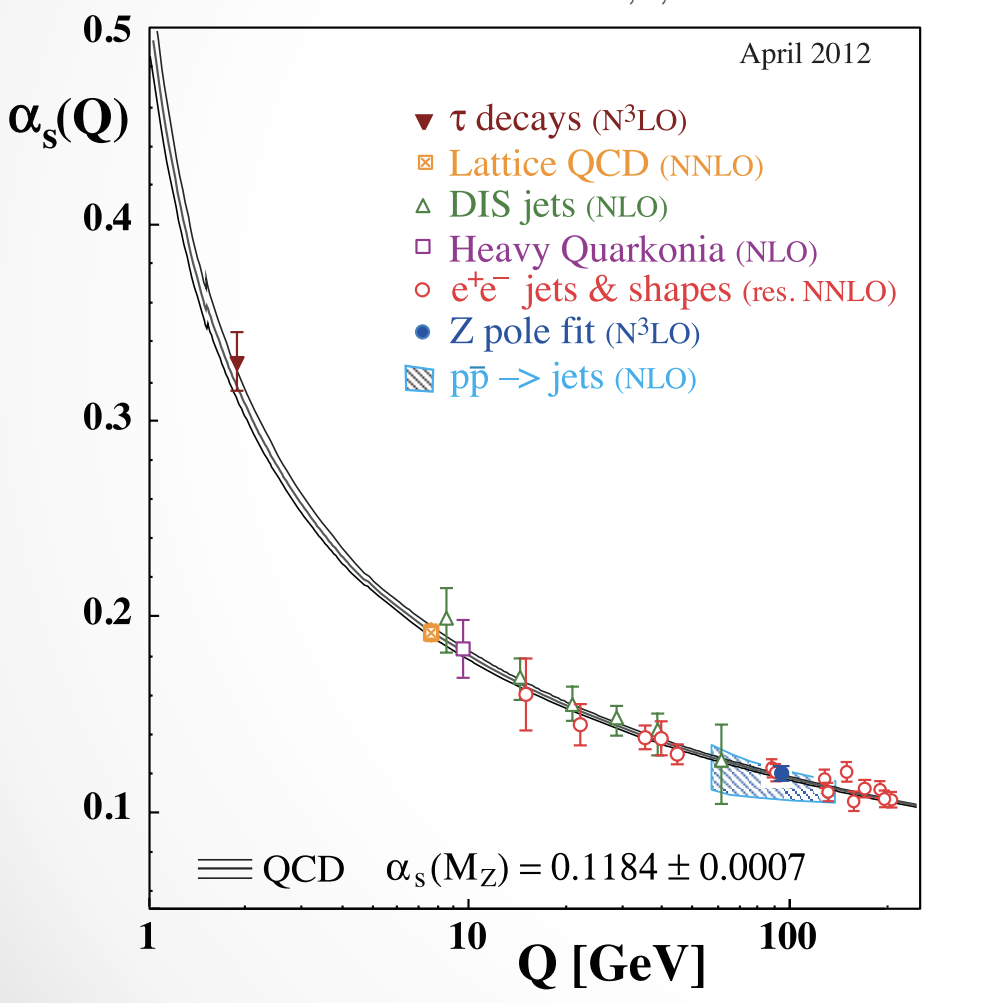
\includegraphics[width=0.6\linewidth]{sm_qcd_coupling}
\caption{Measured values of the strong coupling constant $\alpha_s$ and its predicted values across a range of energies}
\label{fig:sm_qcd_coupling}
\end{figure}

\section{Phenomenology}\label{sec:sm_pheno}

\section{Limitations}\label{sec:sm_limits}
